% This is "sig-alternate.tex" V2.0 May 2012
% This file should be compiled with V2.5 of "sig-alternate.cls" May 2012
%
% This example file demonstrates the use of the 'sig-alternate.cls'
% V2.5 LaTeX2e document class file. It is for those submitting
% articles to ACM Conference Proceedings WHO DO NOT WISH TO
% STRICTLY ADHERE TO THE SIGS (PUBS-BOARD-ENDORSED) STYLE.
% The 'sig-alternate.cls' file will produce a similar-looking,
% albeit, 'tighter' paper resulting in, invariably, fewer pages.
%
% ----------------------------------------------------------------------------------------------------------------
% This .tex file (and associated .cls V2.5) produces:
%       1) The Permission Statement
%       2) The Conference (location) Info information
%       3) The Copyright Line with ACM data
%       4) NO page numbers
%
% as against the acm_proc_article-sp.cls file which
% DOES NOT produce 1) thru' 3) above.
%
% Using 'sig-alternate.cls' you have control, however, from within
% the source .tex file, over both the CopyrightYear
% (defaulted to 200X) and the ACM Copyright Data
% (defaulted to X-XXXXX-XX-X/XX/XX).
% e.g.
% \CopyrightYear{2007} will cause 2007 to appear in the copyright line.
% \crdata{0-12345-67-8/90/12} will cause 0-12345-67-8/90/12 to appear in the copyright line.
%
% ---------------------------------------------------------------------------------------------------------------
% This .tex source is an example which *does* use
% the .bib file (from which the .bbl file % is produced).
% REMEMBER HOWEVER: After having produced the .bbl file,
% and prior to final submission, you *NEED* to 'insert'
% your .bbl file into your source .tex file so as to provide
% ONE 'self-contained' source file.
%
% ================= IF YOU HAVE QUESTIONS =======================
% Questions regarding the SIGS styles, SIGS policies and
% procedures, Conferences etc. should be sent to
% Adrienne Griscti (griscti@acm.org)
%
% Technical questions _only_ to
% Gerald Murray (murray@hq.acm.org)
% ===============================================================
%
% For tracking purposes - this is V2.0 - May 2012

%\documentclass{sig-alternate}
\documentclass{sig-alternate-2013}
\usepackage{algorithm}
\usepackage{algorithmic}
\usepackage{amssymb}
\usepackage{amsmath}
\usepackage{color}
\newtheorem{theorem}{Theorem}[section]
\newtheorem{proposition}[theorem]{Proposition}
\newtheorem{corollary}[theorem]{Corollary}
\newtheorem{fact}[theorem]{Fact}
\newtheorem{observation}[theorem]{Observation}
\newtheorem{definition}[theorem]{Definition}
\newtheorem{lemma}[theorem]{Lemma}
\newtheorem{claim}{Claim}[theorem]
%% AMS symbols
\usepackage{amssymb}

%% Geometry

\newcommand{\An}[1][n]{\ensuremath{\mathbb{A}^{#1}}} % Affine space
\newcommand{\Pn}[1][n]{\ensuremath{\mathbb{P}^{#1}}} % Projective space


%% Some common rings in maths.

\newcommand{\Complex}[0]{\ensuremath{\mathbb{C}}}
\newcommand{\Real}[0]{\ensuremath{\mathbb{R}}}
\newcommand{\Int}[0]{\ensuremath{\mathbb{Z}}}
\newcommand{\PadicInt}[1][p]{\ensuremath{\mathbb{Z}_{#1}}}
\newcommand{\PadicNum}[1][p]{\ensuremath{\mathbb{Q}_{#1}}}
\newcommand{\GF}[1][p]{\ensuremath{\mathbb{F}_{#1}}}
\newcommand{\Ideal}[1]{\ensuremath{\mathfrak{#1}}}


%% Quantum stuff

\newcommand{\ket}[1]{\ensuremath{\left\vert #1 \right\rangle}}
\newcommand{\bra}[1]{\ensuremath{\left\langle #1 \right\vert}}
\newcommand{\braket}[2]{\ensuremath{\left\langle #1 \vert #2 \right \rangle}}

%% Some common groups in maths

\newcommand{\GL}[2]{\ensuremath{\mathrm{GL_{#1}}\left(#2\right)}}
\newcommand{\SL}[2]{\ensuremath{\mathrm{SL_{#1}}\left(#2\right)}}
\newcommand{\PGL}[2]{\ensuremath{\mathrm{GL_{#1}}\left(#2\right)}}
\newcommand{\PSL}[2]{\ensuremath{\mathrm{GL_{#1}}\left(#2\right)}}
\newcommand{\Sym}[1]{\ensuremath{\mathrm{Sym}\left(#1\right)}}
%% Absolute values

\newcommand{\abs}[1]{\ensuremath{\left\vert#1\right\vert}}
\newcommand{\absp}[2][p]{\abs{#2}_{#1}}

%% Galois theory

\newcommand{\Gal}[1]{\ensuremath{\mathrm{Gal}\left(#1\right)}}

%% Algebraic complexity

\newcommand{\matrixtensor}[3]{\ensuremath{\left\langle #1,#2,#3 \right\rangle}}

%% Misc

\newcommand{\Perm}[1]{\ensuremath{\mathrm{perm}\left(#1\right)}}
\newcommand{\Det}[1]{\ensuremath{\mathrm{det}\left(#1\right)}}
\newcommand{\sgn}[1]{\ensuremath{\mathrm{sgn}\left(#1\right)}}
\newcommand{\transpose}[1]{\ensuremath{#1^{\mathrm{T}}}}
\newcommand{\Aut}[1]{\ensuremath{\mathrm{Aut}\left(#1\right)}}
\newcommand{\GI}[0]{\ensuremath{\mathrm{GI}}}
\newcommand{\AUT}[1][]{\ensuremath{\mathrm{AUT}_{#1}}}
\newcommand{\BCGI}[1]{\ensuremath{\mathrm{BCGI}_{#1}}}
\newcommand{\PWS}[1]{\ensuremath{\mathrm{PWS}_{#1}}}

%\usepackage{hyperref}
%\usepackage{showlabels}

\newfont{\mycrnotice}{ptmr8t at 7pt}
\newfont{\myconfname}{ptmri8t at 7pt}
\let\crnotice\mycrnotice%
\let\confname\myconfname%

\permission{Permission to make digital or hard copies of all or part of this work for personal or classroom use is granted without fee provided that copies are not made or distributed for profit or commercial advantage and that copies bear this notice and the full citation on the first page. Copyrights for components of this work owned by others than ACM must be honored. Abstracting with credit is permitted. To copy otherwise, or republish, to post on servers or to redistribute to lists, requires prior specific permission and/or a fee. Request permissions from permissions@acm.org.}
\conferenceinfo{GECCO'14,}{July 12--16, 2014, Vancouver, BC, Canada.}
\copyrightetc{Copyright 2014 ACM \the\acmcopyr}
\crdata{978-1-4503-2662-9/14/07\ ...\$15.00.\\
http://dx.doi.org/10.1145/2576768.2598274 }

\clubpenalty=10000 
\widowpenalty = 10000




\begin{document}
%
% --- Author Metadata here ---

%\CopyrightYear{2007} % Allows default copyright year (20XX) to be over-ridden - IF NEED BE.
%\crdata{0-12345-67-8/90/01}  % Allows default copyright data (0-89791-88-6/97/05) to be over-ridden - IF NEED BE.
% --- End of Author Metadata ---
% \conferenceinfo{GECCO'14,} {July 12-16, 2014, Vancouver, BC, Canada.}
 %   \CopyrightYear{2014}
  
  %\crdata{TBA}
   % \clubpenalty=10000
    %\widowpenalty = 10000
    
    
\title{Performance of Metropolis Algorithm for the Minimum Weight Code Word Problem} 


\numberofauthors{3} %  in this sample file, there are a *total*
% of EIGHT authors. SIX appear on the 'first-page' (for formatting
% reasons) and the remaining two appear in the \additionalauthors section.
%
\author{
% You can go ahead and credit any number of authors here,
% e.g. one 'row of three' or two rows (consisting of one row of three
% and a second row of one, two or three).
%
% The command \alignauthor (no curly braces needed) should
% precede each author name, affiliation/snail-mail address and
% e-mail address. Additionally, tag each line of
% affiliation/address with \affaddr, and tag the
% e-mail address with \email.
%
% 1st. author
\alignauthor
Ajitha Shenoy K B\\
       \affaddr{Department of Computer Science and Engineering}\\
       \affaddr{Indian Institute of Technology}\\
       \affaddr{Kanpur, India.}\\
       \email{ajith@cse.iitk.ac.in}
% 2nd. author
\alignauthor
Somenath Biswas\\
       \affaddr{Department of Computer Science and Engineering}\\
       \affaddr{Indian Institute of Technology}\\
       \affaddr{Kanpur, India.}\\
       \email{sb@cse.iitk.ac.in}
\alignauthor Piyush P Kurur\\
       \affaddr{Department of Computer Science and Engineering}\\
       \affaddr{Indian Institute of Technology}\\
       \affaddr{Kanpur, India.}\\
       \email{ppk@cse.iitk.ac.in}
}

\date{15 July 2014}

\maketitle

\begin{abstract}
  We study the performance of the Metropolis algorithm for the problem
  of finding a code word of weight less than or equal to $M$, given a
  generator matrix of an $[n,k]$-binary linear code.  The algorithm
  uses the set $\mathcal{S}_k$ of all $k \times k$ invertible matrices
  as its search space where two elements are considered adjacent if
  one can be obtained from the other via an elementary row
  operation (i.e by adding one row to another or by swapping two rows.)
We prove that the Markov chains associated with the
  Metropolis algorithm mix rapidly for suitable choices of the
  temperature parameter $T$. We ran the Metropolis algorithm for a
  number of codes and found that the algorithm performed very well in
  comparison to previously known experimental results.
\end{abstract}

% A category with the (minimum) three required fields
\category{G.1.6}{Optimization}
{Simulated annealing}
\category{G.3}{Probability and Statistics}{Probabilistic algorithms (including Monte Carlo)}
\category{H.1.1}{Systems \& Information Theory}{Information Theory}
%A category including the fourth, optional field follows...
\terms{Theory, Algorithms}
\keywords{Metropolis Algorithm; Minimum weight code word;  
search space; conductance; rapid mixing of Markov chain}

\section{Introduction}

An $[n,k]$ binary linear code is a $k$-dimensional subspace of the
vector space of $n$-dimensional binary vectors, its code words are the
elements of the subspace, and a minimum weight code word of such a
code is a non-zero code word with minimum number of 1's.  (We provide
the formal definitions in the next Section). Such a code can be
succinctly presented by providing a basis of the $k$-dimensional
subspace. The minimum weight code word problem requires one to find a
minimum weight code word, given a basis of the code. This problem is
important for several reasons: a minimum weight code word is a measure
of the error correction capability of the
code~\cite{error-correction}, also, codes with large minimum weight
code words have applications in diverse areas such as
cryptography~\cite{crypto-appl1, crypto-appl2, secret-sharing}, pseudorandom
generators~\cite{pseudo-random, pseudo-random2}.

The problem has been shown to be NP-hard~\cite{Elvin}, moreover, it
remains hard even to obtain a constant factor
approximation~\cite{Dumer}. It is for this reason that researchers
have proposed several probabilistic and heuristic algorithms to find
low weight code words, given a basis of a binary linear code. Examples
are: GA \cite{ref1, ref2, ref4}, hill climbing \cite{ref1,ref2, ref4},
tabu search \cite{ref3}, and ACO \cite{ant}.

We study in this paper the efficacy of the Metropolis algorithm for
solving the problem. Our Metropolis algorithm for an $[n,k]$ code uses
the set of all $k\times k$ invertible binary matrices as its search
space set. Two such elements are considered neighbours if one can be
obtained from the other by an elementary row operation. We prove that
the search space graph has large magnification and use this result to
prove that the family of Markov chains, as defined by the Metropolis
algorithm on an input instance, has a large conductance. It is known
that~\cite{Swagato} the Metropolis algorithm solves a combinatorial
optimization problem like ours in polynomial time if and only if (1)
the associated Markov chain family has high conductance (2) the
probability of the favorable event in the stationary distribution is
high. As our Metropolis algorithm tries to find a code word of weight
less than or equal to $M$, where $M$ is given as an input parameter,
the algorithm will be efficient, in view of the conductance result, if
the probability $p_M$ of getting a code word of weight $M$ is high in
the stationary distribution. A good bound for $p_M$ is difficult to
estimate, this quantity closely related to the weight distribution of
the binary linear codes. Therefore, to understand how well the
Metropolis algorithm works for this problem, we experiment with a few
codes. The codes that we use for our experiments are certain BCH codes
and full dimensional codes of dimensions 50 and 100.  We found that
the Metropolis algorithm performed well for several 
BCH (Bose, Chaudhuri and Hocquenghem) codes~\cite{bch}, even
obtaining the minimum in certain cases.  For the full dimensional
case, where the minimum weight is $1$, the algorithm was able to
converge quickly to a small weight code word. This compares favorably
with previously known experimental results on BCH codes which used
certain other search heuristics. Details are given in
Section~\ref{section-experiments}.

% Given a generator matrix $G$ for an length $n$ binary linear code of
% dimension $k$, finding a minimum weight code word is known to be
% NP-hard~\cite{Elvin}. The minimum weight of a linear code is a
% measure of the error correction capability of the code. Thus, the
% problem is of interest in coding
% theory~\cite{error-correction}. Besides codes with large distance
% have applications in various areas like
% cryptography~\cite{crypto-appl1}, pseudo-random generators
% ~\cite{pseudo-random2} %etc. There exists no polynomial time algorithm
% for solving minimum weight code word problem.  Also there is no good
% polynomial time approximation algorithm which approximate the
% minimum weight code word with constant factor~\cite{Dumer}.
% Researchers have developed several probabilistic and heuristic
% algorithms to find low weight codewords quickly, which are possibly
% close to the least weight of a given code.  Some such algorithms are
% proposed in \cite{Anne,Jeffery,Stern,ref1,ref2,ref3,ref4,ant,sim}.
% We study in this paper the efficacy of the Metropolis algorithm to
% find, given $M$, a code word of weight less than or equal to $M$.
% For $[n,k]$-code, the algorithm uses as its search space, the set
% $\mathcal{S}_k$ of all $k \times k$ invertible matrices, where two
% such matrices are considered neighbours if one can be obtained from
% the other by a single elementary row operation. We prove that the
% search graph defined above has magnification at least $1/2$.

\section{Preliminaries}

\begin{definition}
  \textbf{(Binary Linear Codes)} An $[n,k]$-\emph{binary linear code}
  is a $k$-dimensional vector subspace $C$ of the $n$-dimensional
  vector space $\mathbf{F}_{2}^{n}$ over the finite field
  $\mathbb{F}_2$. The parameter $n$ is called the \emph{length} and
  $k$ the \emph{dimension} of the code $C$.
\end{definition}

A binary linear $[n, k]$-code $C$ can be succinctly described by
giving a basis for it. This is typically done by giving a
\emph{generator matrix} for the code $C$.

\begin{definition}\textbf{(Generator Matrix)}
  A generator matrix for an $[n,k]$ linear code $C$ is a $k \times n$
  matrix $G$ whose rows form a basis for $C$.
\end{definition}

This is called a generator matrix because a vector is a code word if
and only if it is a linear combination of the rows of the generator
matrix.

\begin{definition}\textbf{(Elementary row operations)}
  \label{elementary-operation}
  For a $k\times n$ matrix $G$ over the field $\mathbb{F}_2$ with rows
  $\mathbf{g}_r$, $1 \leq r \leq k$, the following are the elementary
  row operations for distinct $i$ and $j$.
  \begin{enumerate}
  \item $\mathbf{g}_i \leftarrow \mathbf{g}_i + \mathbf{g}_j$ (the
    $j$-th row is added to the $i$-th row),
  \item $\mathbf{g}_i \leftrightarrow \mathbf{g}_j$ (rows $i$ and $j$
    are interchanged).
\end{enumerate}
\end {definition}

\begin{definition}{\bf (Minimum weight code word)}
  For a code $C$, a non-zero vector $\mathbf{v} \in C$ of minimum
  Hamming weight is called a minimum weight code word. The
  \emph{minimum weight code word} problem is to compute, given a
  generator matrix $G$ of an $[n,k]$-code $C$, a minimum weight code
  word of $C$.
\end{definition} 

The decision version of the minimum weight code word problem can be
stated as follows.

\begin{definition}\textbf{(Decision version)}
  Given $G$, a generator matrix for $C$ and an integer $M$,
  \emph{decide} whether there exists a non-zero vector in $C$ of
  weight $M$ or less.
\end{definition}  

\section{Search Space}

In this section, we define the search space which we use in our
Metropolis algorithm. Our search space is similar to the search space
defined for shortest lattice vector problem~\cite{ajith, ajith-j}.
The algorithm attempts to construct a generator matrix which has a
minimum weight code word as one of its rows. It is easy to see that
such a generator matrix always exists.

\begin{fact}\cite{linear-algebra}
  Let $G$ be a generator matrix of the $[n,k]$ binary linear code $C$,
  then $G'$ is a generator matrix for $C$ if and only if there is a
  $k\times k$ invertible matrix $U$ such that $G' = UG$.
\end{fact}

Consequently, for any input generator matrix $G$, the set of all
matrices $UG$ as $U$ varies over $k \times k$ invertible matrices is
precisely the set of all generator matrices of $C$.  Therefore, the
search space of our Metropolis algorithm will be the set
$\mathcal{S}_k$ of all $k \times k$ invertible matrices and given a
generator matrix $G$ of $C$ as input, our goal is to find a matrix $U$
in $\mathcal{S}_k$ such that $UG$ contains a minimum weight code word
as one of its rows. A natural neighbourhood structure on the search
spaces $\mathcal{S}_k$ can be defined in terms of elementary row
operations on matrices in $\mathcal{S}_k$. We now formally define our
search space.

\begin{definition}{\bf(Search Space)}\label{sp-defn}
  Given an $[n,k]$-code $C$ via a generator matrix $G$ we define the
  search space as follows.
  \begin{description}
  \item [Elements:] The elements of the search space $\mathcal{S}_k$
    are the $k \times k$ invertible matrices $U$ over $GF(2)$.
  \item[Neighbourhood:] For a matrix $U$ in $\mathcal{S}_k$, the set
    $N(U)$ of neighbours consists of matrices $V$ that can be obtained
    from $U$ by any of the following elementary operations:
    \begin{enumerate}
    \item add the $j$-th row to the $i$-th row,
    \item swap the $i$-th and $j$-th rows,
    \end{enumerate}
    where $i$ and $j$ are two distinct rows of $U$.  This makes the
    underlying graph a $D$-regular graph where $D$ is $k(k-1)$.
  \item[Cost:] For an element $U$ of the search space, the cost
    $c(U)$ is defined to be $w^\alpha$ where $w$ is the minimum of
    the Hamming weights of rows of $UG$ and $\alpha$ is a parameter
    which takes positive values.
  \end{description}
\end{definition}

{\bf Convention:} The elementary row operations that we defined above
can be carried out on a matrix $A$ by post multiplying by a suitable
elementary matrix say $E$. We often identify a row operation with the
corresponding elementary matrix.  Note that $|\mathcal{S}_k|$ equal to
number of binary $ k \times k$ invertible matrices which is less than
$2^{k^2}$, the total number of $k \times k$ binary matrices.

We now show that the diameter of the search space graph is bounded by
a polynomial in $k$.


\begin{proposition}\label{prop-path}
  For any two matrices $U$ and $V$ in the search space $\mathcal{S}_k$
  there is a path between them in the search space graph of length at
  most $k^2$.
\end{proposition}
\begin{proof}
  The matrix $V^{-1}U$ is invertible as both $U$ and $V$
  are. Therefore, $V^{-1}U$ can be transformed to the $k\times k$
  identity matrix $I_k$ by Gauss-Jordan elimination which uses a
  sequence of elementary row operations. This is done in $k$-stages
  one for each column. In the $i$-th stage, we transform the $i$-th
  column to the vector $\mathbf{e}_i$ which has a $1$ at the $i$-th
  position and $0$'s elsewhere. Each of these stages can be carried
  out using at most $k$ elementary row operations (more details in the
  proof of Lemma~\ref{lem-magnification}) and thus using $\ell \leq k^2$
  elementary operations, $V^{-1}U$ gets transformed into $I_k$. Let
  $E_1,\ldots, E_\ell$ be the elementary matrices associated with the
  elementary row operations described above. Consequently, the product
  $V^{-1}U E_1\cdots E_\ell$ is the identity matrix $I_k$. Therefore,
  $V$ is the product $UE_1\cdots E_\ell$.  The sequence of matrices
  $U_i = U \cdot \prod_{j=1}^i E_i$ for $0 \leq i \leq \ell$ gives the
  path from matrix $U = U_0$ to $V = U_\ell$.
\end{proof}

We prove next that our search space graph has large
magnification. This will be used later to show that the family of
Markov chains as defined by our Metropolis algorithm mixes rapidly. We
now recall the definition of magnification~\cite{alistair}. Let $G = (V,E)$
be an undirected graph. Let $S$ be a non-empty subset of $V$ and let
$\overline{S}$ denote its complement, i.e. $V \setminus S$.  Let
$E(S,\overline{S})$ denote the set of edges that go out of $S$. The
magnification $\mu(S)$ is defined as
\[
 \mu(S) = \frac{|E(S,\overline{S})|}{|S|}.
\]

The magnification for the graph $G$ (also called as \emph{edge
  expansion}), denoted by $\mu(G)$, is the minimum $\mu(S)$ where the
minimization is done over all non-empty subsets $S$ of $V$ of
cardinality at most $\frac{|V|}{2}$.

\begin{lemma}
  \label{lem-magnification}
  A search space graph for minimum weight code word problem has
  magnification at least $\frac{1}{2}$.
\end{lemma}
\begin{proof}
  We use the \emph{canonical path
    method}~\cite{cannonical-path-reference} to lower-bound the
  magnification of the search graph. For this, we first canonize the
  Gauss-Jordan elimination procedure described in the proof of
  Proposition~\ref{prop-path} that transforms an arbitrary $k\times k$
  invertible matrix $A$ to identity matrix. The procedure works in
  $k$-stages. The $i$-th stage starts with a matrix $A_{i-1}$ whose
  $r$-th column, for any $r < i$ is the vector $\mathbf{e}_r$, the
  vector which has a $1$ at $r$-th entry and $0$ every where else. In
  the $i$-th stage, we convert the $i$-th column into $\mathbf{e}_i$
  using elementary row operations. The stage begins with a swap of
  $i$-th row if and only if the $(i,i)$-th entry of $A_{i-1}$ is a
  $0$. In such a case, we choose to swap the $i$-th row and the $j$-th
  row, where $j$ is the smallest integer greater than $i$ such that
  the $(j,i)$-th entry is $1$. There is always one such $j$ because
  the matrix $A_{i-1}$ is invertible. Having ensured that the
  $(i,i)$-th entry is 1, we convert each $1$ in the $i$-th column,
  except the $(i,i)$-th entry to 0 by adding the $i$-th row. This
  gives us the matrix $A_i$. The elimination process ends when $i$ is
  $k$ and the resulting matrix $A_k$ becomes identity. Let us call the
  sequence $E_1,\ldots,E_\ell$ of elementary operations used to reach
  the identity matrix from $A$ in the above process as the
  \emph{canonical Gauss-Jordan sequence} associated with the matrix
  $A$.

  We show that canonical Gauss-Jordan sequences satisfy the following
  properties.

  \begin{claim}\label{claim-gauss-jordan}
    \begin{enumerate}
    \item There is a unique canonical Gauss-Jordan sequence associated
      with a given $k\times k$ invertible matrix-$A$. Moreover, two
      distinct matrices $A$ and $A'$ in $\mathcal{S}_k$ will have
      distinct canonical Gauss-Jordan sequences.
    \item The number of distinct canonical Gauss-Jordan sequences is
      equal to the cardinality of the search spaces $\mathcal{S}_k$.
    \item If $E_1,\ldots,E_\ell$ is the canonical Gauss-Jordan
      sequence of some $k\times k$ matrix-$A$, then no two operators
      $E_r$ and $E_s$ in the sequence are the same.
    \end{enumerate}
  \end{claim}
   \begin{proof}
     The way in which we have canonize the Gauss-Jordan elimination
     procedure above, it is clear that there is a unique canonical
     Gauss-Jordan sequence associated with a given $k \times k$
     invertible matrix $A$. Now suppose that two distinct matrices $A$
     and $A'$ in $\mathcal{S}_k$ have the same canonical Gauss-Jordan
     sequence, i.e $AE_1 \ldots E_\ell=I$ and $A'E_1 \ldots E_\ell=I$
     which implies $A=A'=IE_{\ell}^{-1}\ldots E_1^{-1}$ which is a
     contradiction. Hence two distinct invertible matrices $A$ and
     $A'$ will have distinct canonical Gauss-Jordan sequences.  This
     completes the proof of part 1 of our claim. To prove part 2
     notice that the number of distinct canonical Gauss-Jordan
     sequences is equal to the number of invertible matrices in
     $\mathcal{S}_k$ which is equal to $|\mathcal{S}_k|$.  Finally to
     prove part 3, consider any elementary row operation that occurs
     in the canonical Gauss-Jordan sequence. Either it is a row
     addition or a swap of two rows. It is clear that all the row
     additions are distinct as we add the row $i$ only in the $i$-th
     stage of the procedure and that too to distinct rows in the
     $i$-th stage. A swap is used only to convert a $0$-diagonal entry
     to $1$. Consider such swap between rows $i$ and $j$ where $j >
     i$. This swap can happen only at the $i$-th stage and not at the
     $j$-th stage because to convert a $0$ in the diagonal we use a
     row that is lower down in the matrix. This completes the proof of
     part 3.
   \end{proof}

   We now define the canonical path between two search graph elements
   $U$ and $V$ as follows: Let $E_1,\ldots,E_\ell$ be the canonical
   Gauss-Jordan sequence associated with the matrix $V^{-1} U$. Then
   the canonical path from $U$ to $V$ is the sequence $U=
   U_0,\ldots,U_\ell = V$ where $U_i = U \cdot \prod_{j=1}^i
   E_i$. Given $U$ and $V$, by a slight abuse of notation, the
   canonical Gauss-Jordan sequence associated with $V^{-1}U$ is also
   called the \emph{canonical Gauss-Jordan sequence associated with
     the canonical path}\footnote{We note that two different canonical
     paths may have the same associated Gauss-Jordan sequences: The
     canonical paths from $U$ to $V$ and from $U'$ to $V'$ will have
     the same associated canonical Gauss-Jordan sequence if and only
     if $U' = A U$ and $V' = A V$ for some invertible $k\times k$
     matrix $A$} from $U$ to $V$.

  Fix two neighbours $C$ and $D$ in the search space $\mathcal{S}_k$.
  We now estimate the number of canonical paths that go through the
  edge $(C,D)$.

  \begin{claim}\label{claim2}
    For two neighbours $C$ and $D$ in $\mathcal{S}_k$ consider any
    canonical Gauss-Jordan sequence $E_1,\ldots,E_\ell$ containing the
    matrix $C^{-1}D$. There is a unique canonical path through the
    edge $(C,D)$ that has $E_1,\ldots,E_\ell$ as its associated
    canonical Gauss-Jordan sequence.
  \end{claim}
  \begin{proof}
    Consider any canonical Gauss-Jordan sequence $E_1,\ldots,E_\ell$
    such that $E_r = C^{-1}D$ for some $1 \leq r \leq \ell$. By
    Claim~\ref{claim-gauss-jordan} all operators $E_s$, $s \neq r$,
    are different from $C^{-1}D$. Therefore, the only canonical path
    that passes through the edge $(C,D)$ and has $E_1,\ldots,E_\ell$
    as its associated canonical Gauss-Jordan sequence starts at $U =
    CE_{r-1}^{-1}\ldots E_1^{-1}$ and ends at $V = DE_{r+1}\ldots
    E_\ell$.
  \end{proof}

  We have the following consequence of the above claim.

  \begin{claim}\label{claim-bound-canonical}
    Let $C$ and $D$ be neighbours in the search space
    $\mathcal{S}_k$. Then the number of canonical paths passing
    through the edge $(C,D)$ is bounded by the total number of points
    in the search space $\mathcal{S}_k$.
  \end{claim}
  
  This is because such a canonical path is uniquely determined by
  its canonical Gauss-Jordan sequence. The number of distinct Gauss-Jordan
  sequences is equal to the number of $k\times k$ invertible matrices
  which is the number of elements of the search space.

  We now prove the bound on the magnification as given in the
  statement of the Lemma~\ref{lem-magnification}. Consider any
  non-empty subset $S$ such that $|S| \leq \frac{|
    \mathcal{S}_k|}{2}$.  There are $|S| \times |\overline{S}|$
  canonical paths that go from $S$ to $\overline{S}$.  Each of these
  paths passes through one of the edges in $E(S,\overline{S})$. As no
  edge can have more than $ |\mathcal{S}_k|$ canonical paths passing
  through it by Claim~\ref{claim-bound-canonical}, we have $
  |\mathcal{S}_k| \times | E(S, \overline{S})| \geq |S| \times
  |\overline{S}|$.  As $| \overline{S}| \geq
  \frac{|\mathcal{S}_k|}{2}$ we have $| \mathcal{S}_k| \times | E(S,
  \overline{S})| \geq | S| \times
  \frac{|\mathcal{S}_k|}{2}$. Therefore, the magnification $\mu (S) =
  \frac{|E(S,\overline{S})|}{|S|}$ is greater than $1/2$ for all $S$
  of cardinality at most $|\mathcal{S}_k|/2$. Since magnification
  $\mu_k$ of the search space $\mathcal{S}_k$ is the minimum over all
  such $\mu(S)$'s, we have $\mu_k \geq \frac{1}{2}$. This completes
  the proof of Lemma~\ref{lem-magnification}.
\end{proof}

%%%%%%%%%%%%%%%%%%%%%%%%%%%%%%%%%%%%%%%%%%%%%

\section{Mixing time analysis}

We use the Metropolis algorithm for the minimum weight code word
problem. On a given input instance $G$, the Metropolis algorithm runs
a Markov chain: the state space of the chain is the set
$\mathcal{S}_k$ of $k\times k$ invertible matrices, which is the search
space of our problem. Recall that the cost $c(U)$ associated with a
search space element $U$, a matrix, is $w^\alpha$ where $w$ is the
minimum Hamming weight of the rows of $UG$. The Markov chain makes use
of this cost function to define a random walk biased towards code
words of lower weights. We now define the transition probabilities
$p_{UV}$, the probability of making a transition to $V$ given that the
chain is at $U$.
\[
p_{UV} = 
\begin{cases}
  0  & \textrm{if }U \neq V, V \notin N(U) \\
   %%%%%%%
  \frac{1}{2D}\cdot \min
  \left(1,
    \exp\left({\frac{c(U)-c(V)}{T}}\right)
  \right) & \textrm{if }V \in N(U)\\
  %%%%%%% 
    1 - \sum_{W\neq U} p_{UW}      &  \textrm {if }U = V.
\end{cases}
\]

In the above definition $T$ stands for the temperature parameter,
which remains fixed for the algorithm, and $D$ is the degree of the
underlying regular graph $\mathcal{S}_k$. Recall that $D$ is
$k(k-1)$.  It is well known~\cite[Chapter:
10.4.1]{citation-for-metropolis} that the above Markov chain has the
stationary distribution given by
\[
\pi_U = \frac{\exp\left({\frac{-c(U)}{T}}\right)}{\sum_{V \in \mathcal{S}_k}
  \exp\left({\frac{-c(V)}{T}}\right)}.
\]


The complete algorithm (Algorithm \ref{algo-metropolis}) is given below:

 \begin{algorithm} 

   \caption{Metropolis Algorithm}  \label{algo-metropolis}
 \begin{algorithmic}[1]

   \STATE \text{Input : The generator matrix $G$ of linear code
     $C$} and an integer $M$

   \STATE \text{Output : Matrix $U$ such that $UG$ contains a vector $\mathbf{v}$} with
   $w_{H}(\mathbf{v}) \leq M $.

 Let $U$ be the starting state in the search space as in Definition \ref{sp-defn}
 and $c(U)$ denote its cost.
 \STATE \text{Set $BestWeight=c(U)$, steps=0}
 \WHILE{$BestWeight > M$ \text{ and } $steps < TSteps$ \\
 \text{[$TSteps$ denotes Max. No. of steps specified by user]}}
 \STATE \text{Select any one of the neighbour $U$ of $V$ uniformly at} \\
 \text{random by performing one of the elementary } \\
\text {operations as defined in Definition \ref{sp-defn}}

 \STATE \text{Set $U = V$ with probability} \[\alpha = \frac{1}{2}.\min\left( \frac{\exp\left(\frac{-c(V)}{T}\right)}{\exp\left(\frac{-c(U)}{T}\right)} , 1\right)\]
 \IF{$BestWeight > c(U)$}
 \STATE $BestWeight =c(U)$
 \ENDIF 
 \STATE $steps=steps+1$;
 \ENDWHILE	
 \end{algorithmic}
 \end{algorithm} 

We now show that the above Markov chain has large conductance for an
appropriate choice of the temperature parameter $T$.

\begin{definition}{\bf(Conductance)\cite{alistair}}
  For any non empty subset $S$ of states in $\mathcal{S}_k$ with non
  empty complement $\overline{S}$, the \emph{conductance} $\phi(S)$ of
  $S$ is defined as 
  
  \[ 
  \phi(S) = \frac{F_S}{C_S}
  \] where

  %\begin{equation}
  \[
    C_S=\sum_{U \in S} \pi_U
  \]
  %\end{equation}

  %\begin{equation}
  \[  F_S=\sum_{U\in S, V \in \overline{S}}p_{UV}\pi_U \]
  %\end{equation}

  The \emph{conductance} $\phi_k$ of the Markov chain is defined to be
  %\begin{equation}
 \[   \phi_k = \min_{S: C_S \leq \frac{1}{2}} \phi(S)  \]
%\end{equation}
\end{definition}


It is easy to see that $F_S=F_{\overline{S}}$ for all such sets $S$.
This implies that $\phi(\overline{S}) = \phi(S) \frac{C_S}{1-C_S}$ (since 
$C_S + C_{\overline{S}} = \sum_{U \in \mathcal{S}_k} \pi_U = 1$ which implies
$C_{\overline{S}} = 1 - C_S$), so
we may equivalently write
%\begin{equation}
 \[ \phi_k = \min_{S} \{\max(\phi(S), \phi(\overline{S}))\} \]
%\end{equation}

\begin{theorem}
  \label{theorem-conductance} The conductance $\phi_k$ of the Markov
  chain associated with our Metropolis algorithm for solving the
  minimum code word problem for an $[n,k]$-code satisfies
  \[
  \phi_k \geq \frac{1}{4D\exp{\left(\frac{2(n^\alpha-1)}{T}\right)}},
  \] 
  where $T$ is the temperature parameter and $\alpha$ is the exponent
  used in the cost function. In particular, when $T=\Omega(n^\alpha)$
  the conductance is $\Omega\left(\frac{1}{D}\right)$, where
  $D$-denotes the number of neighbours for a node in the search graph.
\end{theorem}
\begin{proof}
  Consider any non-empty subset $S$ of $\mathcal{S}_k$ such that $C_S
  \leq \frac{1}{2}$. There are two possibilities: either $ |S| \leq
  \frac{|\mathcal{S}_k|}{2}$ or $ |S| > \frac{|
    \mathcal{S}_k|}{2}$. We handle these cases separately.
  
  First assume that $ |S| \leq \frac{| \mathcal{S}_k|}{2}$. The flow
  out of $S$ is bounded as follows.
  \begin{displaymath}
  F_S = \sum_{U\in S, V \in \overline{S}}p_{UV}\pi_U
  \geq  \min(p_{UV})\min(\pi_U)|E(S, \overline{S})| 
\end{displaymath}

By Lemma ~\ref{lem-magnification}, our search graph has magnification at
least $1/2$ and hence $|E(S,\overline{S})| \geq \frac{1}{2}|
S|$. As a result we have:
\begin{equation}
  \label{eq3}
  F_S \geq \min(p_{UV})\min(\pi_U)\frac{| S| }{2}.
\end{equation}
We know that:
\begin{displaymath}
  \pi_U = \frac{\exp\left({\frac{-c(U)}{T}}\right)}
  {\sum_{V \in \mathcal{S}_k}\exp\left({\frac{-c(V)}{T}}\right)} 
  = \frac{\exp\left({\frac{-c(U)}{T}}\right)}{Z}.
\end{displaymath}
where $Z$ is the partition function $\sum_{V \in
  \mathcal{S}_k}\exp\left({\frac{-c(V)}{T}}\right)$.  Let $c_{\max}$ and
$c_{\min}$ denote the maxima and minima of the cost function $c(.)$
respectively. Notice that $c_{\max} \leq n^\alpha$ and $c_{\min} \geq
1$. Therefore, for any element $U$ of the search space, its stationary
probability $\pi_U$ is bounded above and below as follows.
\begin{equation}
  \frac{\exp\left({\frac{-n^\alpha}{T}}\right)}{Z} 
  \leq \pi_U 
  \leq \frac{\exp\left({\frac{-1}{T}}\right)}{Z}
  \label{eq4}
\end{equation}

Also, the transition probabilities $p_{UV}$ satisfies
\begin{equation}
  p_{UV} 
  \geq \frac{1}{2D\exp\left({\frac{c_{\max}-c_{\min}}{T}}\right)} 
  \geq \frac{1}{2D\exp\left({\frac{n^\alpha-1}{T}}\right)}.
\label{eq5}
\end{equation}
From Equations (\ref{eq3}),(\ref{eq4}) and (\ref{eq5}) we obtain
\begin{equation}
  F_S 
  \geq \frac{\exp\left({\frac{-n^\alpha}{T}}\right)}{Z} \cdot
  \frac{1}{2D\exp\left({\frac{n^\alpha-1}{T}}\right)} \cdot \frac{|S| }{2}
\label{eq6}
\end{equation}

The capacity $C_S$ is bounded as follows:
\begin{equation}
 C_S = \sum_{U \in S}\pi_U 
     \leq \max(\pi_U) \cdot |S| 
     =     \frac{\exp\left({\frac{-1}{T}}\right)}{Z} \cdot |S|
 \label{eq7}
 \end{equation}
 Therefore from Equations (\ref{eq6}) and (\ref{eq7}), the conductance $\phi(S)$ of the subset $S$ is lower
 bounded as:
 \begin{equation}\label{eqn-phis}
   \phi(S) = \frac{F_S}{C_S} \geq 
   \frac{1}{4D\exp\left({\frac{2(n^\alpha-1)}{T}}\right)}
 \end{equation}

 Now consider the case when $|S| > \frac{|\mathcal{S}_k|}{2}$.  Using
 Equation (\ref{eqn-phis}) for $\overline{S}$, we obtain:
 \[
 \phi(\overline{S}) \geq \frac{1}{4D\exp\left({\frac{2(n^\alpha-1)}{T}}\right)}.
 \]

 Since $C_{\overline{S}} \geq \frac{1}{2}$ and
 $\frac{C_{\overline{S}}}{1-C_{\overline{S}}} \geq 1$, we have:
 \[
 \phi(S)
 =\frac{C_{\overline{S}}}{1-C_{\overline{S}}} \phi(\overline{S}) 
 \geq \frac{1}{4D\exp\left({\frac{2(n^\alpha-1)}{T}}\right)}
 \]

 Thus, we find that for both the cases, \emph{viz.}, $|S| \leq \frac{|
   \mathcal{S}_k|}{2}$ and $|S| > \frac{|\mathcal{S}_k|}{2}$,
 \[
 \phi(S) \geq \frac{1}{4D\exp\left({\frac{2(n^\alpha-1)}{T}}\right)}.
 \]
 As a result, the conductance $\phi_k$ of the Markov chain
 is bounded by
 \[
 \phi_k  \geq \frac{1}{4D\exp\left({\frac{2(n^\alpha-1)}{T}}\right)}.
 \]
\end{proof}



We use the above conductance result to show that the Markov chain for
the Metropolis algorithm mixes rapidly, i.e., in time polynomial in
$n$ for an input $[n,k]$-code. Let $P^t(U_0,.)$ denote the probability
distribution obtained by running the Markov chain for $t$ steps
starting the chain at $U_0$. As before $\pi$ denotes the stationary
probability distribution.  To define mixing time we need the concept
of total variation distance.

\begin{definition}{\bf{Total Variation Distance}\cite{david}}
  Total variation distance between two probability distributions
  $P^t(U_0,.)$ and $\pi$ is defined as:
  \[
  ||P^t(U_0,.)-\pi||_{TV} = \frac{1}{2} \cdot \sum_{V \in
    \mathcal{S}_k}|P^t(U_0,V)- \pi(V)|
  \]
\end{definition} 

The mixing time $\tmix$ of the Markov chain is defined as

\begin{displaymath}
  \tmix = \min\{t: \Delta(t)  \leq \varepsilon\},
\end{displaymath}
where $\Delta(t)= \max_{U_0 \in \mathcal{S}_k}||P^t(U_0,.)-\pi||_{TV}$
denotes maximal variation distance between $P^t(U_0,.)$ and $\pi$ as
$U_0$ varies over the elements of the search space
$\mathcal{S}_k$\cite{david}. In other words, independent of the choice
of the initial state $U_0$ to start the chain, if we run the Markov
chain for $t \geq \tmix$ steps, we have the guarantee that in the
resulting distribution, the probability $P^t(U_0,U)$ of obtaining the
any state $U$ is bounded above and below as follows.

%\begin{equation}\label{eqn-probability-bounds}
\[  \pi_U - \varepsilon \leq P^t(U_0,U) \leq \pi_U + \varepsilon. \]
%\end{equation}

A lower bound on the conductance $\phi_M$ of a Markov chain $M$
translates to an upper bound on the mixing time as
follows~\cite[Equation (2.13), page 58]{alistair}.

\begin{equation}
  t_{\mathrm{mix}}^M(\varepsilon) 
  \leq \frac{2}{\phi_M^{2}} 
  \left( \ln{\varepsilon^{-1}} + 
    \ln{\pi_{\min}^{-1}} \right).
  \label{eqn-mixing-time}
\end{equation}
where $\pi_{\min}$ denotes the smallest of the stationary
probabilities for the chain $M$ and $t_{\mathrm{mix}}^M(\varepsilon)$
denotes its mixing time. Using Theorem~\ref{theorem-conductance} we
obtain the following bound on mixing time.

\begin{corollary}
  \label{tmixo}
  The mixing time $\tmix$, of the Markov chain associated with our
  Metropolis algorithm on an input $[n,k]$-code satisfies:
  \[
  \tmix 
  \leq 32D^{2}\exp{\left(\frac{4(n^\alpha-1)}{T}\right)}
  \cdot (k^2 \ln2 + \frac{n^\alpha-1}{T} + \ln \varepsilon^{-1}),
  \]
  where $D$ is the number of neighbours of any search point which we
  know to be $k(k-1)$.  

  In particular, when the temperature parameter $T$ is $\Omega(n^\alpha)$,
  the mixing time $\tmix$ is $O(k^6 + k^4 \ln \varepsilon^{-1})$.
\end{corollary}
\begin{proof}
  We first derive a bound on the probability $\pi_{\min}$ as follows.
  For any element $U$, we have
  \begin{displaymath}
    \pi_U = \frac{\exp\left({\frac{-c(U)}{T}}\right)}{\sum_{V \in \mathcal{S}_k}\exp\left({\frac{-c(V)}{T}}\right)}.
  \end{displaymath}
  Using the bound $ 1 \leq c(U) \leq n^{\alpha}$ for the cost function
  $c(.)$, we obtain the following.
  \begin{displaymath}
    \pi_U 
    \geq \frac{\exp{\left(\frac{-n^\alpha}{T}\right)}}
    {\sum_{V \in \mathcal{S}_{k}}\exp\left({\frac{-1}{T}}\right)} 
    = \frac{1}{\exp\left({\frac{n^\alpha-1}{T}}\right)| \mathcal{S}_k|}.
  \end{displaymath}

  The set $\mathcal{S}_k$ is the set of all $k\times k$ invertible
  matrices and hence $|\mathcal{S}_k| \leq 2^{k^2}$. Thus:
  \begin{equation}\label{eqn-pi-min}
    \pi_{\min} \geq \frac{1}{2^{k^2}\exp\left({\frac{n^\alpha-1}{T}}\right)}.
  \end{equation}
  Therefore, $\ln \pi_{\min}^{-1} \leq k^2 \ln2 +
  \frac{n^\alpha-1}{T}$.

  The result follows from the above, Equation (\ref{eqn-mixing-time}),
  and the bound on conductance given in
  Theorem~\ref{theorem-conductance}.
\end{proof}

Given the generator matrix $G$ of an $[n,k]$-code $C$ and a bound $M$,
our task is to find a code word of Hamming weight $M$ or less if it
exists. Every run of the Metropolis algorithm for $\tmix$ steps
provides us with a sample $U$ with probability at least $\pi_U -
\varepsilon$. By taking the row of minimum weight in $UG$, we get a
sample code word $\mathbf{x}$ of $C$. Let $p_M$ be the probability
that the sample code word $\mathbf{x}$ is of weight less than or equal
to $M$. Then we have:
\[
p_M \geq \sum_{U: \mathrm{wt}(UG) \leq M} (\pi_U - \varepsilon),
\]
where $\mathrm{wt}(UG)$ denotes the minimum of the Hamming weights of
the rows of the matrix $UG$.

We take $S$ samples $\mathbf{x}_1,\ldots, \mathbf{x}_S$ obtained
through $S$ runs of the Metropolis algorithm each for $\tmix$ time and
choose the one with the least Hamming weight. The probability that we
fail to find a code word of weight $M$ or less is upper bounded by
$(1-p_M)^S$. Therefore, to obtain the such a code word with
probability at least $\delta$, we need $S \geq \frac{\log(1 -
  \delta)}{\log(1 - p_M)}$.

Let $N_M(G)$ denote the number of $k \times k$ invertible matrices $U$
such that $UG$ has a row of Hamming weight less than or equal to $M$.
Choosing $\varepsilon = \frac{1}{2} \cdot \pi_{\min}$, we get $p_M$ to
be greater than $\frac{1}{2} \cdot N_M(G) \cdot \pi_{\min}$. Further,
setting the temperature $T$ to $n^\alpha$ we obtain, the mixing time
$\tmix$ to be $O(k^6)$ (Corollary~\ref{tmixo}) and $\pi_{\min}$ to be
$\frac{1}{e2^{k^2}}$ (Equation (\ref{eqn-pi-min})). Using these values,
we have a bound on the total time $\ttotal$ as
\[
\ttotal = S \cdot \tmix = O\left( k^6 \cdot \frac{\log(1 - \delta)}{\log(1
  - p_M)}\right).
\]
where $p_M$ is $O\left(\frac{N_M(G)}{2^{k^2}}\right)$.

For a fixed code $C$ if $G$ and $G'$ are two generator matrices of $C$
we have $G' = U G$ for some $U$ in $\mathcal{S}_k$. Therefore, $N_M(G)
= N_M(G')$. As a result $N_M(G)$ is an invariant of the code $C$. We
do not have an analytical expression for it. It is closely related to
the well studied weight distribution function of the code.

The above discussions show that our algorithm will be able to find a
code word of weight $M$ or less in polynomial time if $N_M(G)$ is
large at most a polynomial factor away from $2^{k^2}$. Since we do not
have a closed form expression for $N_M(G)$ for most codes, we run
experiments to see how the algorithm performs on typical binary linear
codes.

\section{Experimental Results} \label{section-experiments}

In the previous section, we proved that for the cost function $c(U) =
\mathrm{w}^\alpha$, the family of Markov chains associated with
the Metropolis algorithm is guaranteed to mix rapidly if we set the
temperature $T$ as $n^\alpha$. To understand the performance as
$\alpha$ varies, we performed experiments on two BCH codes
BCH(511,58,183) and BCH(511,184,91) and the trivial $[50,50,1]$ and
$[100,100,1]$ codes with $\alpha$ set as $1/2$, 1, 2, 3, 5 and 7. We
chose the trivial codes because their minimum weight code words are
known: they are code words with a single 1. For $BCH(n, k, d)$ codes
$d$ stands for the \emph{design distance} (see Section 7.3 in ~\cite{bch-design-distance}) and it lower bounds the actual
minimum weights. The performance is plotted in Figure~\ref{alpa} in
which we observe that the performance is best for $\alpha =1$. With
$\alpha$ set to $1$, we tested our algorithm on the set of 20 test
cases given in six previous
publications~\cite{ref1,ref2,ref3,ref4,ant,sim}. The heuristic search
algorithms used in these publications are Wallis's
GA~\cite{ref1,ref2}, Askali's GA~\cite{ref1,ref4},
Tabu-search~\cite{ref1, ref2, ref3, ref4}, Hill
Climbing~\cite{ref1,ref2, ref4}, Ant colony optimization~\cite{ant}
and simulated annealing\cite{ant, sim}. Each of these heuristics use the
same set, namely, the set of all length $k$ binary words, as their
search space. 

We report the comparison of our algorithm against the algorithms cited
above in Table~\ref{t3}, where the last two columns report the
performance of our algorithm. The last but one column is for the case
when our algorithm is run for $k^2$ steps and the best of $5000$
samples is chosen. In the last column, we do the same with
$500$-steps, taking the best of $2000$ samples. The other columns in
the Table~\ref{t3} give the performance of the previously studied
algorithms.  Based on the result, it can be seen that our Metropolis
algorithm outperforms hill climbing, tabu search, Wallis's genetic
algorithm and ant colony optimization \cite{ref1,ref2,ref3,ref4,ant}
in all the twenty cases considered.  When compared to the Askali's
genetic algorithm~\cite{ref4, ref1} on the twenty test cases, the
performance was same in 9 cases, the genetic algorithm outperforms our
algorithm in 4 test cases and our algorithm outperforms the genetic
algorithm in 7 test cases.
% So we win \vfill\eject

% We compared our algorithm with previously developed search heuristics
% defined in \cite{ref1, ref2,ref3,ref4,ant,sim}.  Note that search
% space used by these heuristics are different from our search space.
% Our search space is set of all $k \times k$ invertible matrices over
% $GF(2)$, where search space used by other heuristics are set of all
% $k$ length vector over $GF(2)$.  Search space used by our algorithm is
% some what similar to the search space used for shortest lattice vector
% problem (SVP) in ~\cite{ajith, ajith-j}.  Detailed description of
% search space and the heuristic algorithms are found in \cite{ref1,
%   ref2,ref3,ref4,ant,sim}.

% We have tested our
% algorithm on binary BCH codes~\cite{bch}. Binary BCH codes were
% discovered by Hocquenghem in 1959 and by Bose and Chaudhuri in 1960.
% Hence it is called as BCH codes.  They are example for binary linear
% codes.  If $n=2^m -1$ and $n-k \leq mt$ then minimum weight($d_{min}$)
% of a binary BCH code is greater than or equal to $2t+1$, where $m$ and
% $t$ are integers such that $m \geq 3$ and $t < 2^{m-1}$.  So we have
% considered $[n, k, d]$ binary BCH codes where $d = 2t+1$ denotes the
% design distance and $d_{min} \geq d$. 

% Results obtained for the 20 test cases using different search
% heuristics (other than our algorithm) is not recomputed and it is
% taken from their respective publications\cite{ref2,ref3,ref4,ant,sim}.
% Hill Climbing and Tabu Search use maximum of 20,000 steps but no
% improvement found after 100 steps.  Askali's GA and Wallis's GA uses
% 10,000 populaton size and searches at most 1,000,000 solutions over 75
% generation. 


We also compared the performance of our algorithm with that of the
simulated annealing as reported in \cite{ant}. The paper~\cite{ant}
considered two BCH codes namely BCH(127, 64, 21) and BCH(255, 91, 51)
and obtained code words of weight 27 and 75 respectively. In
comparison, our algorithm was able to attain the minimum weight as 21
and 55 respectively.

\begin{figure*}
\centering
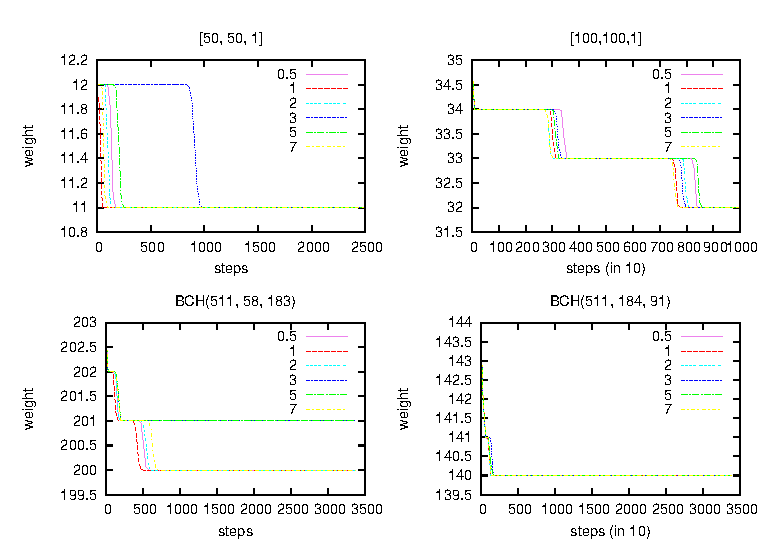
\epsfig{file=t-al.eps, height=4.25 in , width =7  in}
%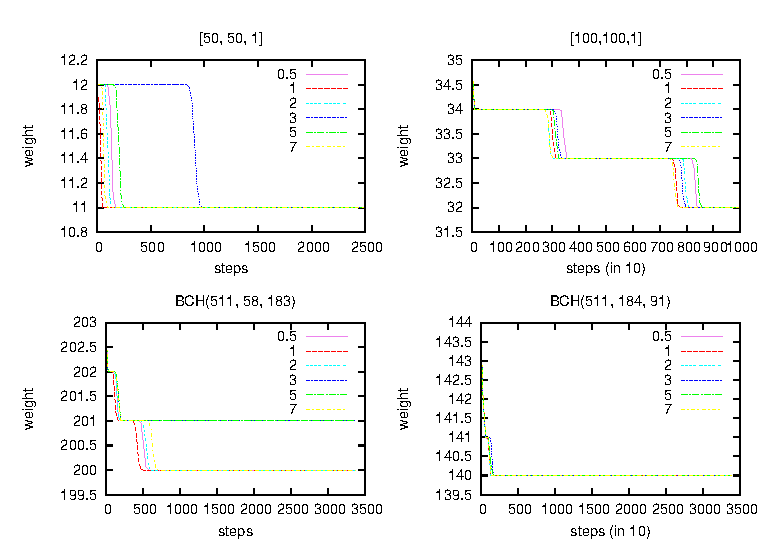
\epsfig{file=t-al.eps}
\caption{Varying $\alpha$ to choose best $\alpha$: $\alpha$ set as
  0.5, 1, 2, 3, 5 and 7 ($k^2$ steps, Average is taken over 1000
  samples)}
\label{alpa}
\end{figure*}



\begin{table*}
\caption{Minimum Weight Code word found using  Our Metropolis Algorithm  
Vs Different Methods given in papers~\cite{ref1, ref2, ref3, ref4, ant}}
\label{t3}
\centering
\begin{tabular}{llllllll}
\hline
\noalign{\smallskip}
\centering
Codes BCH & Askali's  & Wallis's  & Hill & Tabu & Ant Colony&Metropolis& Metropolis \\
$(n, k, d-design)$ & GA & GA & Climbing & Search & Optimization& Our Method & Our Method\\
&\cite{ref1, ref4} &\cite{ref1, ref2} & \cite{ref1, ref4, ref2} 
&\cite{ref3, ref1, ref4, ref2} & \cite{ant}&$k^2$ steps & 500 steps\\
&&&&&&5000 Samples&2000 samples\\
\noalign{\smallskip}

\hline
\noalign{\smallskip}

BCH (127, 64, 21) & \bf{21} & \bf{21} & 28 & 24 & 24& \bf{21}&\bf{21}\\
\hline
BCH (127, 57, 23) & \bf{23} & \bf{23} & 28 & \bf{23}  &24& \bf{23}&\bf{23}\\
\hline
BCH (127, 50, 27) & \bf{27} & \bf{27} & 32 & 31 & \bf{27}&\bf{27}& \bf{27} \\
\hline
BCH (255, 71, 59) & \bf{63} & 66 & 79 & 79 & 70&\bf{63}&64\\
\hline
BCH (255, 79, 55) & \bf{57} & 60 & 74 & 64 & 69&\bf{57}&\bf{57}\\
\hline
BCH (255, 87, 53) & \bf{57} & \bf{57} & 70 & 66 & 66&\bf{57}&\bf{57}\\
\hline
BCH (255, 91, 51) & \bf{53} & 59 & 72 & 69& 68&54&54\\
\hline
BCH (255, 99, 47) & \bf{51} & 55 & 64 & 61 & 62 &\bf{51}&52\\
\hline
BCH (255, 107, 45)& \bf{49} & 51 & 64 & 62 & 60&50&50\\
\hline
BCH (255, 115, 43)& \bf{45} & 50 & 57 & 55 & 58&46&46\\
\hline 
BCH (511, 304, 51) &74 & 79 & 90 & 85 &--&\bf{73}&74\\
\hline
BCH (511, 286, 55) &84&84&96&92&--&\bf{78}&82\\
\hline
BCH (511, 238, 75)&103&105&118&112&--&102&\bf{99}\\
\hline
BCH (511, 220, 79) &109&111&123&117&--&\bf{108}&\bf{108}\\
\hline
BCH (511, 184, 91)& \bf{111}&128&135&140&--&120&127\\
\hline
BCH (511, 166, 95)&135&137&152&140&-- &131&\bf{128}\\
\hline
BCH (511, 121, 117)&155&152&163&163&--&151&\bf{148}\\
\hline
BCH (511, 103, 123)&\bf{160}&164&179&179&--&\bf{160}&\bf{160}\\
\hline
BCH (511, 76, 171)&176&176&195&184&--&\bf{171}&175\\
\hline
BCH (511, 58, 183)&\bf{183}&185&207&199&--&\bf{183}&\bf{183}\\
\hline
\end{tabular}
\end{table*}




\section{Conclusion}

In this paper, we studied the performance of the Metropolis algorithm
for the minimum weight code word problem for binary linear codes. For
an $[n,k]$-code, the algorithm uses a search space consisting of
$k\times k$ invertible matrices and two such matrices are considered
neighbours if one can be obtained from the other by an elementary row
operation. We prove that the magnification of the search graph is
large. Since this is the property of the search space, other random
search heuristics can also possibly use the same search space
profitably. Using the magnification result, we also prove that the
Markov chain associated with a problem instance has large conductance,
which is a necessary condition for the Metropolis algorithm to preform
well on that instance. As simulated annealing (SA) has a close
connection to the Metropolis algorithm, it would be instructive to try
SA for this problem on our search space. We performed experiments to
see how well does our algorithm perform on certain codes as against
previously studied heuristics for the problem.  The experimental
results show that our algorithm performs quite well, it out-performs
several previous heuristic algorithms used for this problem.

%
% The following two commands are all you need in the
% initial runs of your .tex file to
% produce the bibliography for the citations in your paper.
\bibliographystyle{abbrv}
\bibliography{mybib}  % sigproc.bib is the name of the Bibliography in this case

% You must have a proper ".bib" file
%  and remember to run:
% latex bibtex latex latex
% to resolve all references
%
% ACM needs 'a single self-contained file'!
%
%APPENDICES are optional
%\balancecolumns
\end{document}
